The implementation of The Onion Router was first described by the U.S. Navy Research Laboratory, as means to protect government communications from digital, as well as physical attacks, by hiding the location of the communicating party or parties \cite{goldschlag1996hiding}.

In 2002, it was decided to ditch the old code base and reimplement the project as Tor, the Second Generation Onion Router, introducing perfect forward secrecy, directory servers, hidden services and more \cite{dingledine2004tor}. In this section, we will explain the various compoments of Tor such as Onion Routing, the structure of the network, circuit creation and disadvantages of Tor.

\subsection{Onion routing}
	As described in the original design paper of The Onion Router, network traffic is forwarded through a circuit of nodes, where each node only knows the previous and next node in the circuit. With a sufficiently long circuit of (independent) nodes, this means that two communicating parties can remain oblivious of each others physical location.
				
	Say we have a circuit consisting of four nodes: our trusted client node ($C$), an (entry or guard) relay node ($X$), a (middle) relay node ($Y$) and an exit node ($Z$). In this case, there are three relay nodes, but this is not a fixed number. A visualisation of this path can be seen in figure \ref{fig:tor_layout}. Each node has its own public key and a corresponding private key. When building the circuit, our client generates a distinct secret for each of these nodes. More information about the circuit setup, can be found in II-D. Circuit creation.
				
	The payload of each packet flowing through the circuit is first encrypted with the distinct secret for last node $Z$, then with the distinct secret for node $Y$, and last with the secret for node $X$. With each layer of encryption, a header is added with the address of the next node in the circuit, plus the used distinct secret encrypted with corresponding nodes public key. 
				
	After node $X$ receives this packet from out trusted node $C$, it decrypts the attached secret with its private key, and uses that secret to decrypt the rest of the packet. The result is a header with the address for node $Y$ and the payload encrypted with secrets for the following nodes in the circuit, which is forwarded to node $Y$.
				
	As a node receives a packet from the previous node, it peels off another layer of encryption, much as how you can peel an onion layer for layer, and forwards it to the next node in the circuit (as specified in the decrypted header). When exit node $Z$ decrypts the last layer, it forwards the unencrypted payload outside the network to the original destination that our trusted client $C$ tried to contact, acting as a traditional proxy.
				
	When exit node $Z$ receives a response, this whole process is applied in reverse order, encrypting the payload with its secret along the way, instead of decrypting. When our client $C$ receives the packet, it peels off all the encryption layers to retrieve the unencrypted payload.
	
	With the second generation onion routing used in Tor, a modified algorithm is used to derive the encryption keys, called \emph{telescoping path-building}, which also provides perfect forward secrecy. This algorithm is described in section \ref{ss:tor_circuit}.
	
	\begin{figure}[!t]
		\centering
		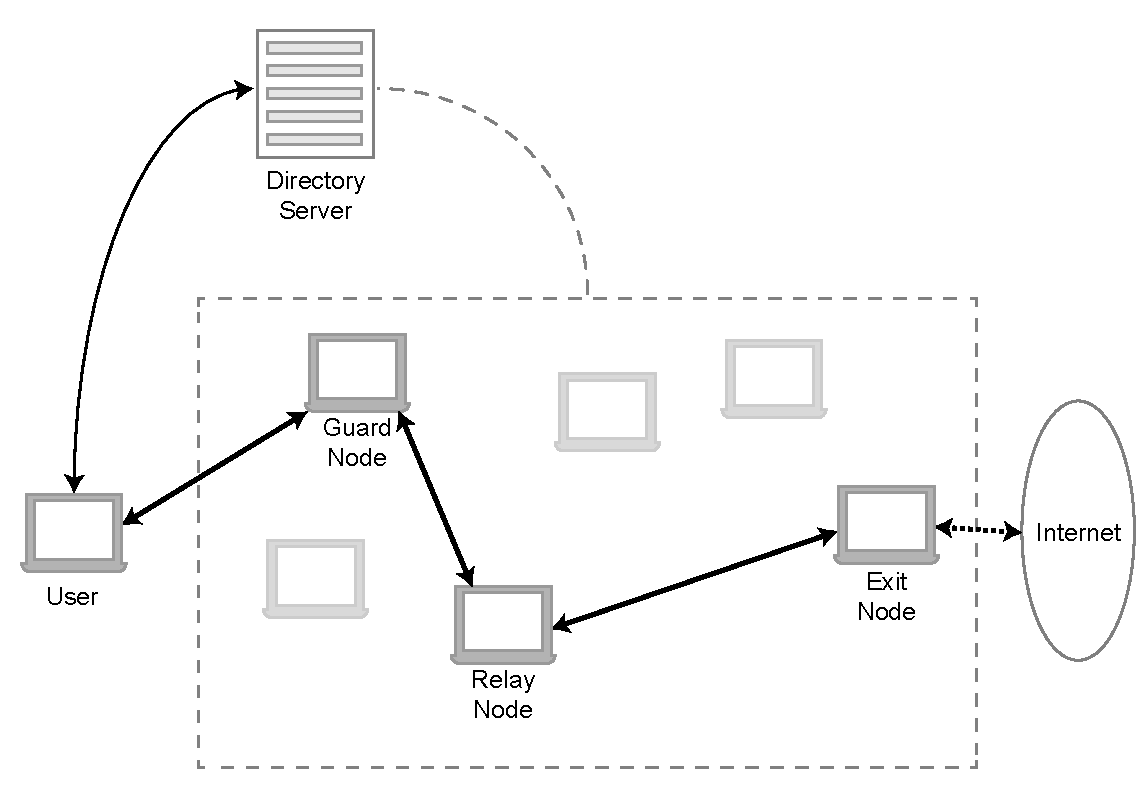
\includegraphics[width=0.4\textwidth]{graphics/tor.pdf}
		\caption{The components of the Tor network. After downloading the node list from the Directory Server, the user creates a circuit through a guard node, a relay node and an exit node, and uses it to communicate (anonymously) with the internet.}
		\label{fig:tor_layout}
	\end{figure}
			
\subsection{Directory servers}
	The original Onion Router implementation used in-band status updates where each node broadcasts know nodes to its neighbours. An attacker could exploit this to isolate and limit the knowledge of a client, forcing connections through malicious nodes. Beside possible security disadvantages, in-band status updates also have the disadvantage that it takes longer to propagate throughout the network and create a global consensus.
				
	To mitigate these concerns, Directory Servers were introduced to Tor during its reimplementation to keep a redundant central consensus about the network. They act as HTTP servers to which Tor nodes can publish signed information about themselves. Tor clients can in turn download this information, as seen in figure \ref{fig:tor_layout}.
				
	This information is signed by the Directory Servers before it is distributed to the Tor clients. The keys to verify these signatures are preloaded in the Tor software, along with the list of Directory Servers, which implies trust by the Tor client in the Directory Servers.

\subsection{Relay and exit nodes}
	The Tor network consists of several components. The clients in the Tor network are known as Onion Proxies. The software to run an Onion Proxy is available for free on the Tor website \cite{torprojectwebsite} and is easy for users to configure. The Onion Proxies are responsible for downloading the directory information, establishing circuits across the network and handling connections from user applications.
	
	The routing in the network is done by Onion Routers, also called relay nodes. The relay nodes relay the data from the Onion Proxy to the web server across a circuit (circuits are described in II-D). Each Onion Router is connected to every other Onion Router with a TLS connection \cite{tlsprotocol}. Each circuit has three type of Onion Routers \cite{mccoy2008shining}:
	
	\begin{itemize}
		\item{The entrance Tor router:} this router is directly connected to an Onion Proxy and can observe the origin of a request through the Tor network. The entrance router sends the packet to the middle Tor router.
		\item{The middle Tor router:} this router is connected to the entrance router and the exit router.
		\item{The exit Tor router:} this router is connected to the web server. Note that the exit Tor router is the only router that can observe the final destination of the request.
	\end{itemize}
	
	The first router in a circuit is the entrance router. The entrance router sends the data to one of the middle router which forwards the data to the exit router.
		
\subsection{Circuit creation}
	\label{ss:tor_circuit}
	
	As described in the previous section, data on the Tor networks travels over circuits. The data travels over the circuit in fixed-size cells that are 512 bytes long. Each cell has a header and a payload. The header consists of a number that identifies the circuit the cell travels on and a command that indicates what to do with the cell’s payload.
	
	Before a circuit can be established, a path has to be chosen. The current path selection algorithm in Tor selects nodes based on the bandwidth of the nodes [link naar cacr2011-20]. Nodes that have more bandwidth, have a higher probability to be chosen for the circuit setup, however, the same node can't be used more than once in a circuit.
	
	Suppose Alice is an Onion Proxy that wants to connect through the Tor network to a web server. Circuit setup uses the Diffie-Hellman key-exchange protocol \cite{diffiehellman} to establish a shared secret between nodes. To create a new circuit, Alice first sends a \emph{create} cell with the first half of the Diffie-Hellman handshake ($ g^b $) to the first node in her selected path (for example, OR1). OR1 sends a \emph{created} cell back with the second half of the key ($ g^b $) along with a hash of the final key. Now both Alice and OR1 have a shared key they use to encrypt and decrypt data sent between them.
	
	So now Alice has a connection with the first Onion Router in the circuit. To extend the circuit to OR2, Alice first sends a \emph{relay extend} cell to OR1. This cell contains the address of the next Onion Router in the circuit and the first half of the key to use in the communication between her and OR2 ($ g^{a_2} $). OR1 takes this first half of the key and sends a \emph{create} cell with this key to OR2. When OR1 receives a created cell, OR1 passes this cell to Alice. Now Alice and OR2 share a common key: $ K = g^{a_2b_2} $. The same procedure can be used to extend the circuit with more nodes.
		
\subsection{Disadvantages}
	\label{ss:tor_disadvantages}

	While Tor guarantees anonymity, there are some disadvantages using it. The main disadvantage is that the Tor network is slow. According to the Tor Metrics project [link naar tor metrics project], it takes about 6 seconds to download 1 MiB of data.
	
	According to Dingledine et al \cite{dingledine2009performance}, there are six reasons why Tor is not optimal. In this section, we will summarize these reasons and explain what could be done to fix them.
	
	First of all, the congestion control does not work well. The network has some problems handling bulk transfers, such as when downloading large files or streaming high-quality videos. The congestion control could be improved by using an unreliable protocol for links between Tor relays. Goldberg et al. [linkje] have proposed PCTCP which could improve the response time of the Tor network with 60\% and the download time of files with 30\%.	
	
	Some Tor users put more traffic on the network than they contribute by running a Onion Router. This means that these users are slowing the network down as they use more traffic than giving to the network. A possible solution for this is to throttle certain high-bandwidth protocols such as BitTorrent at exit nodes or at Onion Proxies.
	
	Also, the Tor network doesn't have the capacity to handle all the users that want privacy on the Internet. By increasing the amount of Onion Routing in the Tor network, the capacity is increased. Incentives such as LIRA \cite{jansen13lira} could make more users run a Onion Router, thus increasing the capacity of the network and making it faster.		
	
	The current path selection algorithm of Tor doesn't distribute the load evenly over the network. The problem is that the current selection strategy is optimal when the network is fully loaded. This is not always the case. Using a better path selection algorithm could increase the capacity of the network and the overall user experience.		
	
	Another problem is that the Tor clients are not optimal at handling latency and connection failures. For example, if extending a circuit fails, the entire circuit is abandoned. An improvement would be to first try to extend the circuit to some other places. If that fails, the circuit could be abandoned. Also, a better timeout mechanism could be chosen for building circuits.		
	
	Much of the overhead of the network is in downloading the directory information. There is also overhead in the TLS connection between the nodes in the network. According to Dingledine et al, removing the empty TLS application record could reduce the overhead in the TCP/IP header with 6.3\%.
	
	As we saw, the directory service generates overhead on the network. If we could replace this central authority, we could reduce the overhead of the network and improve the performance. This means, we would like to have Tor decentralized. Many research has been done already on the decentralization of Tor [linkjezz] but so far, no anonymous, well-performing decentralized network has come up. This is due to the fact that there are many problems decentralization brings along with.